\documentclass[a4paper, 12pt]{article}
\usepackage{cmap}           % Пакет для поиска в полученной пдфке
\usepackage[utf8]{inputenc} % Ззамена кодировки файла на utf8
\usepackage[T2A]{fontenc}   % Подключение кодировки шрифтов
\usepackage[russian]{babel} % Использование русского языка 
\usepackage[left=2cm, right=2cm, top=1cm, bottom=2cm]{geometry} % Изменение размеров полей
\usepackage{indentfirst}    % Красная строка в начале текста
\usepackage{amsmath, amsfonts, amsthm, mathtools, amssymb, icomma, units, yfonts}
\usepackage{amsthm} % Пакет для нормального оформления теорем
\usepackage{graphicx}
\usepackage{tikz}
\usepackage{esvect}
\usetikzlibrary{calc,matrix}

%Теоремы
\newtheorem*{standartbase}{Теорема о стандартном базисе}
\newtheorem*{fulllemma}{Лемма}
\newtheorem*{sl1}{Следствие 1}
\newtheorem*{sl2}{Следствие 2}
\newtheorem*{monotonousbase}{Теорема о монотонном базисе}
\newtheorem*{scheme}{Утверждение 1}
\newtheorem*{n2}{Утверждение 2}
\newtheorem*{zhegalkin}{Теорема Жегалкина}
\newtheorem*{poste}{Теорема Поста}

\renewcommand{\qedsymbol}{\textbf{Q.E.D.}}

\begin{document}
\title{Дискретная математика. Модуль 3. Лекция 1}
\author{Лекторий ПМИ ФКН 2015-2016\\Бубнова Валерия\\Жижин Пётр\\Пузырев Дмитрий}
\date{11 января 2016}

\maketitle
\section*{Схемы. Булевы схемы}
\textsc{Важное примечание:} В данной лекции все рассмотренные функции являются \textit{всюду определенными}.

\textit{Схема} --- это функция, заданная последовательность присваиваний.

Также в профессиональной среде схемы принято называть SLP (\textit{straight line programmes}). 

Рассмотрим такую функцию $f$, определенную для булевых значений (\textit{булеву функцию}): $f:\{0, 1\}^n \rightarrow \{0, 1\}$.

\textit{Базисом} B булевой функции будем называть некий набор $B:\{f_1, f_2, \ldots , f_n\}$, где $f_1 \ldots f_n$ - булевы функции.

\textit{Булева схема} в базисе B  --- последовательность функций $x_1, x_2, x_3... x_n, x_{n+1} := S_1, x_L := S_{L-n}$, которая вычисляет $x_L(x_1, \ldots ,x_n)$. 

\[S_j = g(S_{i_1},  ... , s_{i_r}), g \in B, i_\mathalpha < j\]

\textit{Стандартный базис} есть базис, состоящий из операций отрицания, конъюнкции и дизъюнкции: $\{\lnot, \vee, \wedge\}$

\textsc{Пример 1}

Зададим булеву схему с помощью стандартного базиса.

$x_1, \ldots ,x_n, s_1 := \lnot x_1, s_2 = \lnot x_2, s_3 := x_1 \wedge s_2, s_4 := x_2 \wedge s_1; s_5 := s_3 \vee s_4$

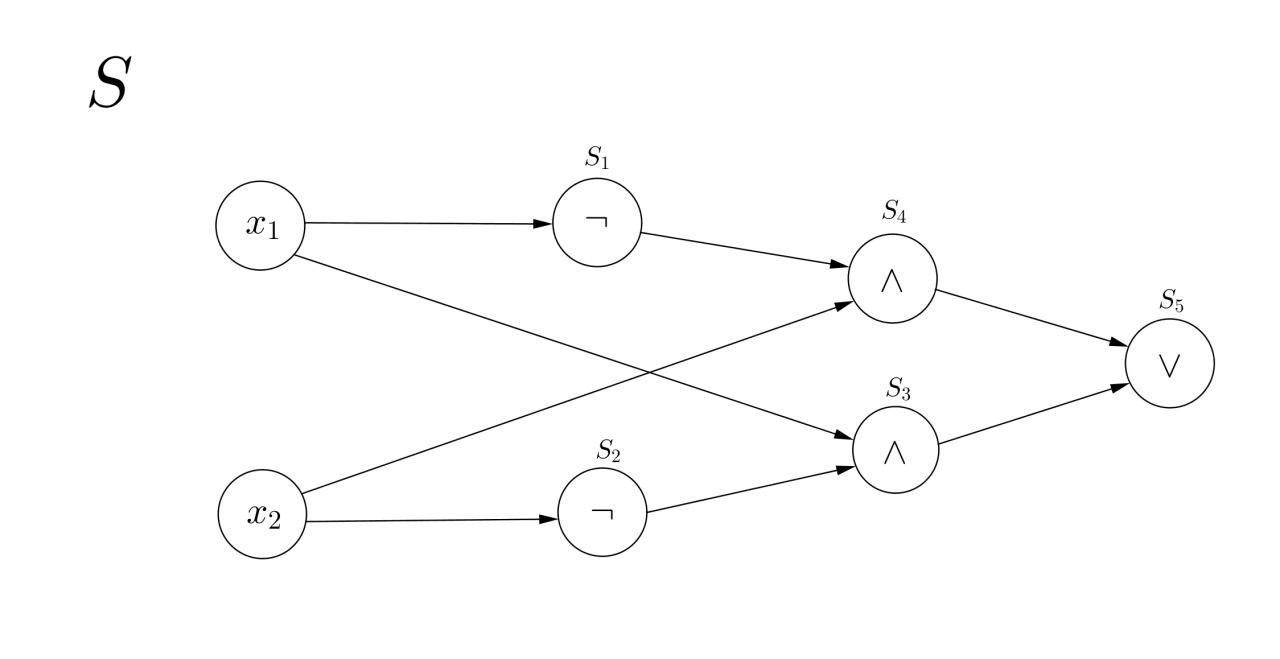
\includegraphics[height=7cm]{images/1.png}
 
 Если $x_2 = 0$, то $s_5 = x_1$
  
 Если $x_2 = 1$, то $s_5 = \lnot x_1$
 
 Результатом выполнения булевой схемы является сложение по модулю 2 (1, если значения $x_1$ и $x_2$ разные) - $\oplus$.
 
 \textsc{Пример 2}
 
 Составим схему, которая является сложением по модулю 2 $n$ переменных. Приведём индуктивное доказательство её существования: 
 
 \begin{enumerate}
     \item База индукции --- $n = 2$. Сложение 2 переменных по модулю 2 возможно по схеме, описанной выше
     \item Предположим существование такой схемы для $n - 1$ переменных 
     \[x_1 \oplus x_2 \oplus \ldots \oplus x_{n-1}\]
     \item Рассмотрим сложение по модулю 2 $n$ переменных. Представим его как сложение по модулю 2 $x_n$ с результатом предыдущего шага. Существование второго слагаемого объясняется предположением индукции. Сложение с $x_n$ можно выполнить по схеме выше. 
     \[x_1 \oplus x_2 \oplus \ldots \oplus x_{n-1} \oplus x_n = (x_1 \oplus x_2 \oplus \ldots \oplus x_{n-1}) \oplus x_n\]
 \end{enumerate}
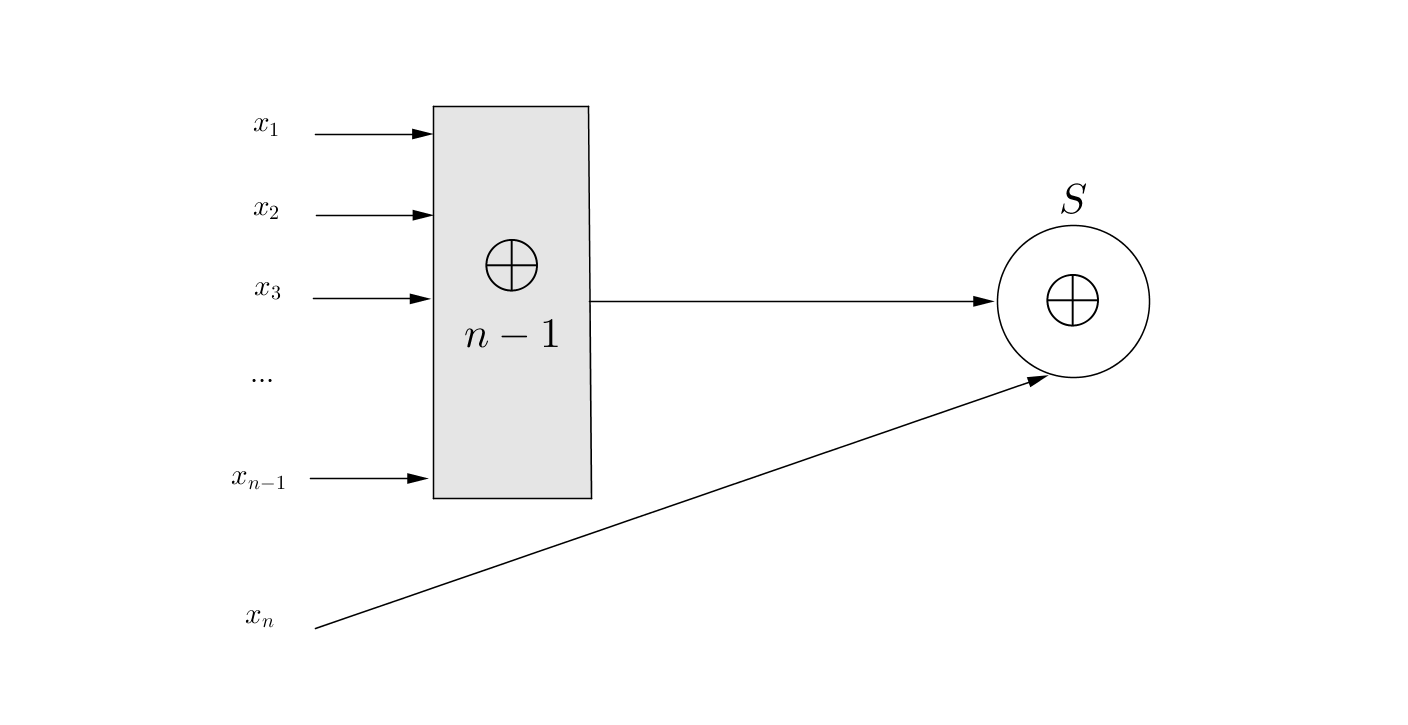
\includegraphics[height=7cm]{images/2.png}
 
 \textsc{Пример 3}
 
 Дизъюнкция n переменных --- аналогично, по индукции. Такие рассуждения можно построить и для конъюнкции.
 
 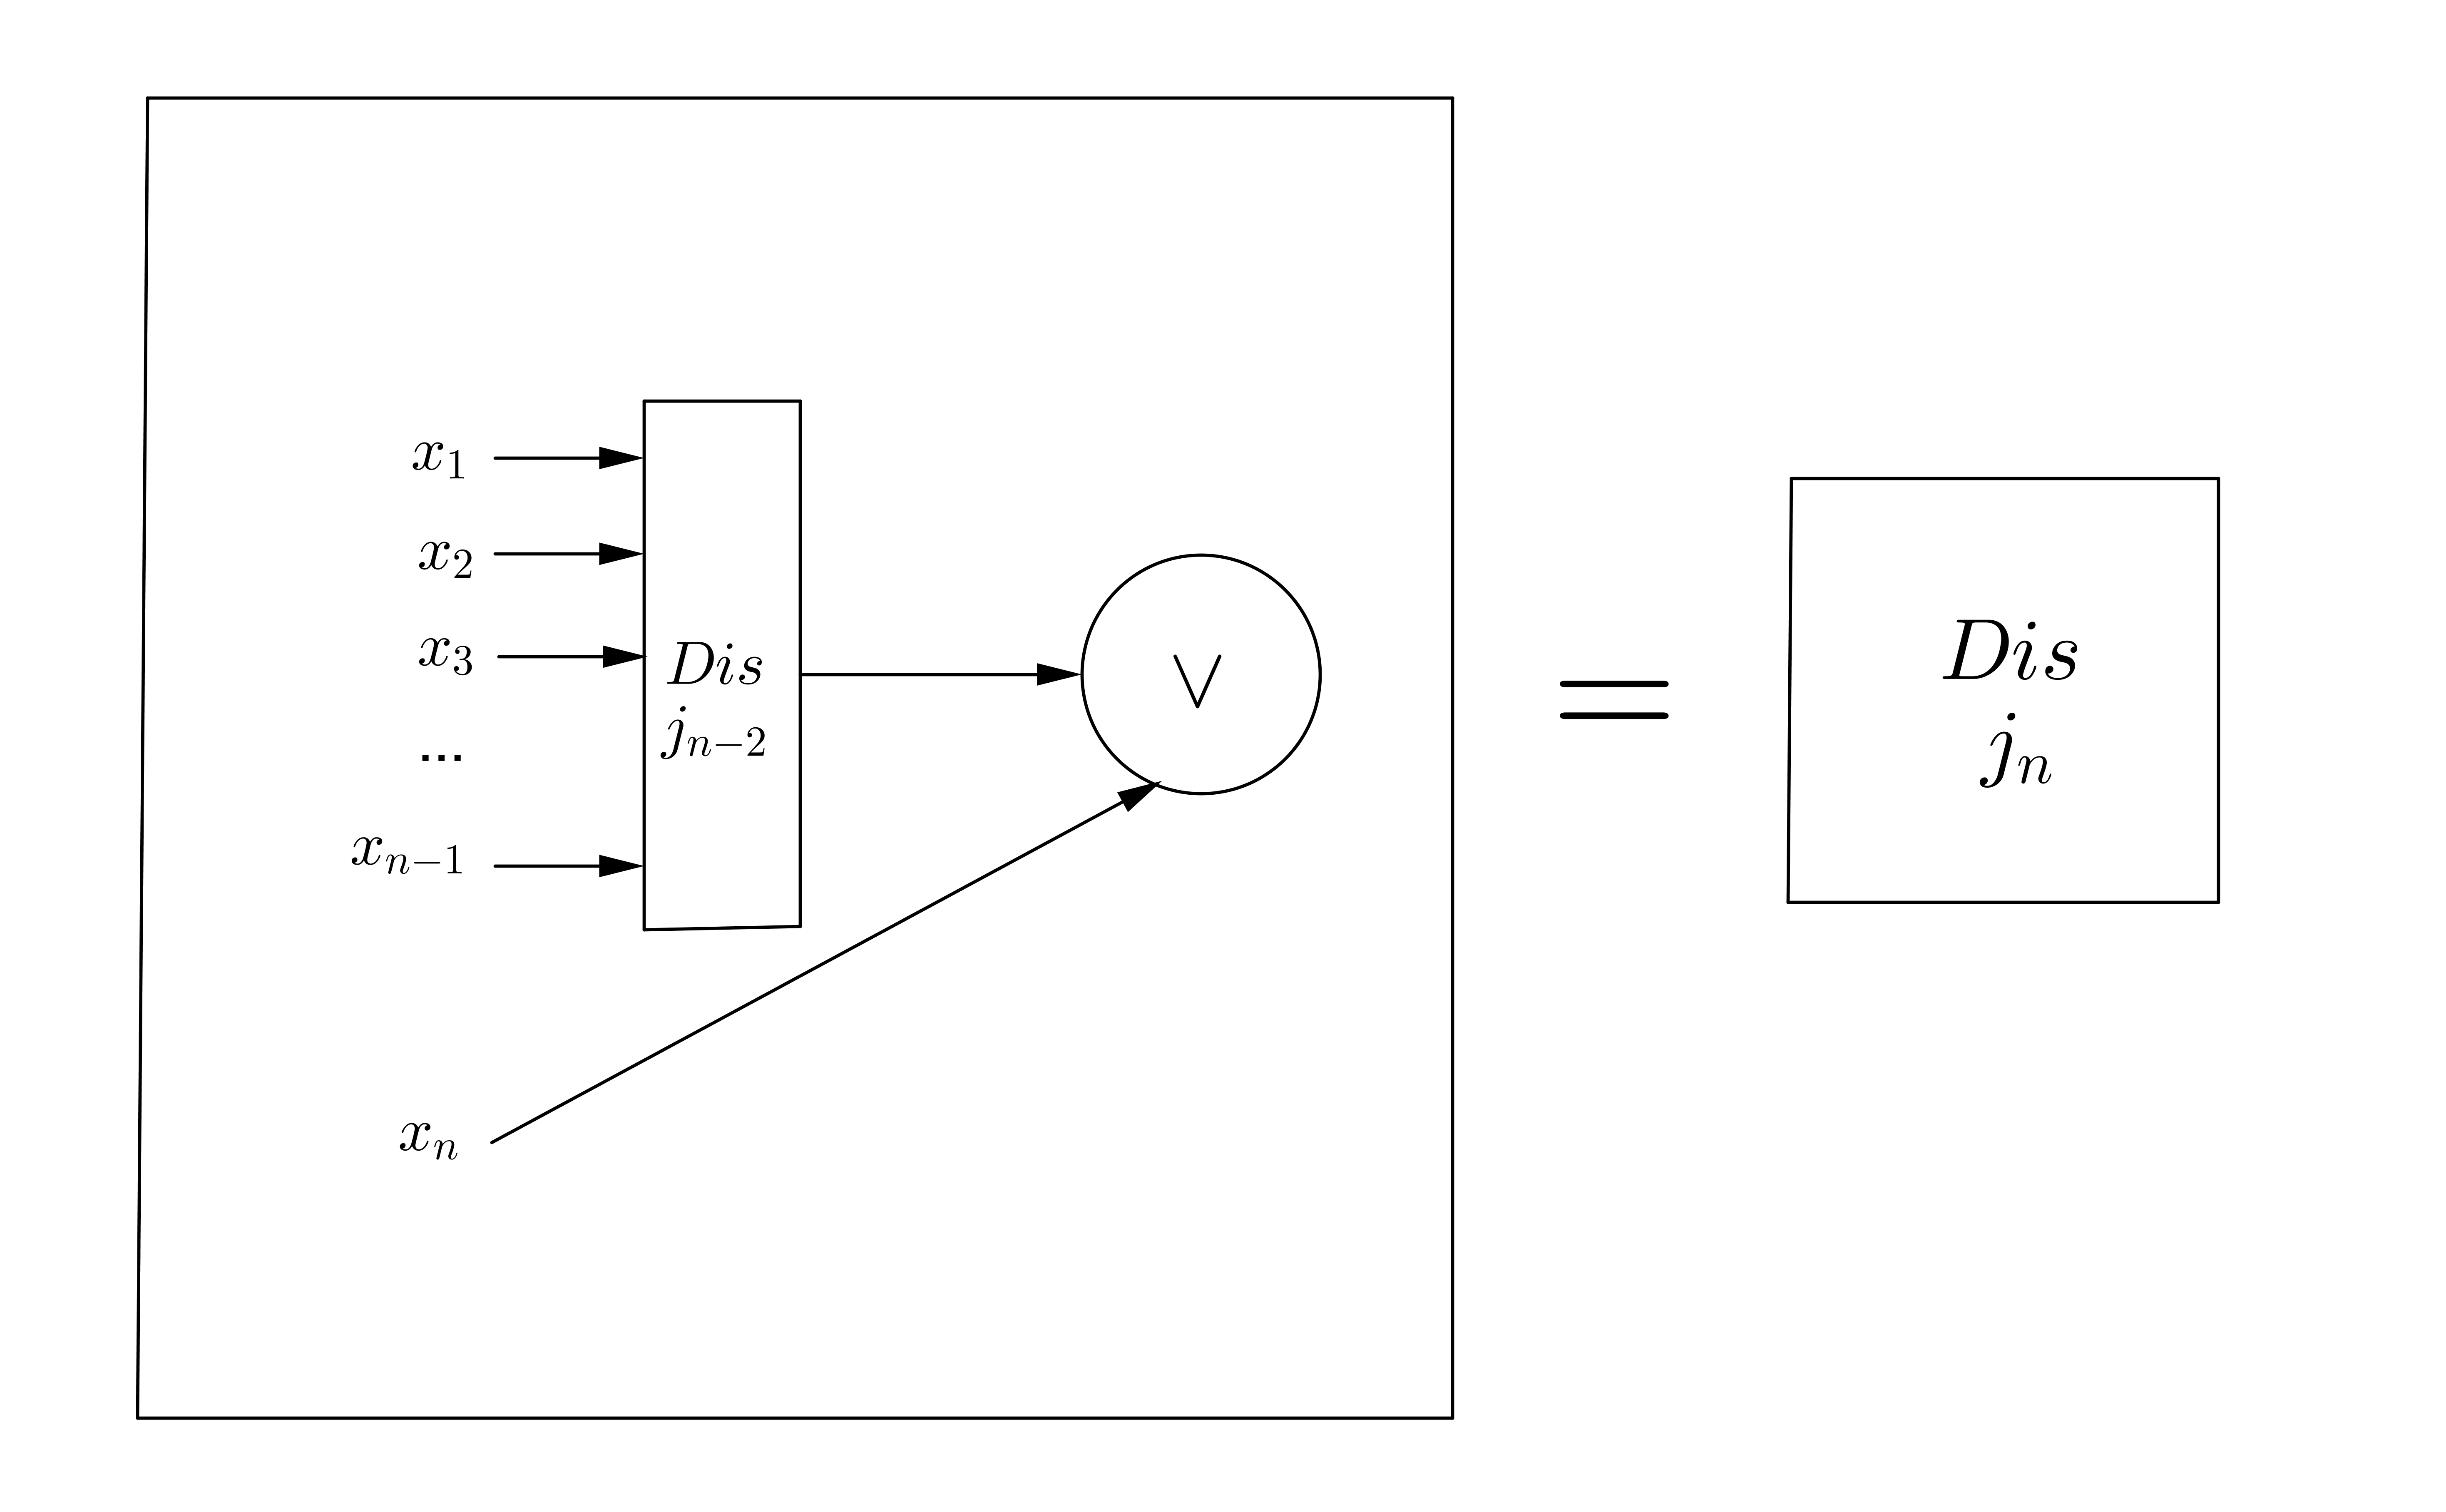
\includegraphics[height=7cm]{images/3.png}
 
 \section*{Анализ схем}
 
 \textit{Анализ базисов: } все ли функции можно выразить через схему в данном базисе?
 
 \textit{Полный базис: } Базис B - \textit{полный}, если любую булеву функцию можно вычислить схемой в базисе B.
 
 \begin{standartbase}
 Стандартный базис --- полный.
 \end{standartbase}
 \begin{proof}
Вспомним, что ДНФ - это дизъюнкция конъюнктов литералов. Построим схему ДНФ.

$x_1, \ldots ,x_n, \lnot x_1, \ldots ,\lnot x_n, c_1, \ldots ,c_n, D$, где $c_j$ --- конъюнкция литералов, D --- дизъюнкция. Данный порядок действий соответствует определению ДНФ, следовательно ДНФ представима в виде схемы и любая функция представима в виде ДНФ. что доказано ранее. (Note: $0 = x \wedge \lnot x, 1 = x \vee \lnot x$)
\end{proof}

 \begin{fulllemma}
Пусть базис $B_1$ --- полный.

$\forall f \in B_1$ вычисляется схемой в базисе $B_2$.

Тогда $B_2$ --- полный.
 \end{fulllemma}
 \begin{proof}
 Вычислим схему в базисе $B_1$.
 
$(B_1) x_1,... x_n,s_j := $вычисление $f, F(..)$

Теперь вычислим схему в базисе $B_2$.

$(B_2) 			   $вычисление $f, F(..)$

\end{proof}
\textsc{Примечание: } Заметим, что если стандартный базис выразим через некоторые функции, то данные функции будут составлять полный базис.

\begin{sl1}
Полнота базиса Жегалкина $\{1, x_1 \wedge x_2, x_1 \oplus x_2\}$.
\end{sl1}
\begin{proof}
$\lnot x_1 = 1 \oplus x_1$ $x_1 \vee x_2 = x_1 \oplus x_2 \oplus (x_1 \wedge x_2)$ или $x_1 \vee x_2 = \lnot (\lnot x_1 \wedge \lnot x_2)$
\end{proof}

\textbf{Немного о схемах.}

Любая формула является схемой. При этом формула --- частный случай схемы. Не любая схема --- формула.

\textsc{Пример: }
$x_1 \oplus x_2 = x_1 \wedge \lnot x_2 \vee \lnot x_1 \wedge x_2 = F
(x_1 \oplus x_2) \oplus x_3 = (F)  \wedge \lnot x_3 \vee \lnot F \wedge x_3$

\begin{sl2}
Полнота базиса {$\lnot, \wedge$}.
\end{sl2}
\begin{proof}
$x \vee y = \lnot (\lnot x \wedge \lnot y)$
\end{proof}
Функция $f:\{0, 1\}^n \rightarrow \{0, 1\}$ называется \textit{монотонной}, если $\forall i: x_i \leqslant y_i \Rightarrow f(x_1 \ldots x_n) \leqslant f(y_1 \ldots y_n)$

\textit{Монотонный базис} --- это базис {$\vee, \wedge$}

\begin{monotonousbase}
Монотонный базис $\{\vee, \wedge\}$ --- неполный
\end{monotonousbase}
\begin{proof}
Воспользоваться монотонностью функций $x_1 \vee x_2$ и $x_1 \wedge x_2$ и немонотонностью функции $\lnot x_1$
\end{proof}
\begin{scheme}
Схема в монотонном базисе вычисляет монотонную функцию.
\end{scheme}
\begin{proof}
Доказываем индукцией по размеру схем
\[x_1, \ldots, x_n, S_1 \ldots S_L, S_{L+1}\] 
\[s_{L+1}:=f(s_{i_1}... s_{i_r})\]
\[S_{i\alpha}(x) \leqslant S_{i\alpha}(y)\]
Так как f --- монотонная
\[S_{L+1}(x) \leqslant S_{L+1}(y)\]
\end{proof}

Заметим также неполноту следующих базисов:
\begin{enumerate}
    \item $\{\wedge,\oplus\}$
    \item $\{1,\wedge\}$
    \item $\{1,\oplus\}$
\end{enumerate}

Функция называется \textit{линейной}, если существуют такие $a_0, a_1, \ldots ,a_n$, где $a_i \in {0;1}, \forall i = \overline{1,n}$ имеет место равенство 
\[f(x_1, \ldots ,x_n) = a_0 \oplus a_1 \wedge x_1 \oplus \ldots \oplus a_n \wedge x_n\]

\begin{n2}
Сумма двух линейных функций также будет линейна.
\end{n2}
\begin{proof}
\[a_0 + \sum a_ix_i + b_0 + \sum b_ix_i = (a_0 + b_0) + \sum (a_i + b_i)x_i\]
\end{proof}

\textit{Полином Жегалкина} представляет из себя сумму по модулю два произведений неивертированных переменных. Формально это можно записать так: $P(x_1 \ldots x_n) = a_0 \oplus${\Large $\oplus_{i = 1}^n$} $a_i \wedge x_i, a_i \in {0,1}$

\textit{Примечание. Не все булевы функции --- линейные}

Линейных функций --- $2^{n+1}$

Булевых функций --- $2^{2^n}$

Получается, линейных функций меньше.

\begin{zhegalkin}
Любая булева функция представима единственным образом в виде полинома Жегалкина.
\end{zhegalkin}
\begin{proof}
 \textit{Существование: }Заметим, что различных булевых функций от n переменных $2^{2^n}$ штук.При этом конъюнкций вида $x_{i_1}\ldots x_{i_k}$ существует ровно $2n$, так как из $n $возможных сомножителей каждый или входит в конъюнкцию, или нет. В полиноме у каждой такой конъюнкции стоит 0 или 1, то есть существует $2^{2^n}$ различных полиномов Жегалкина от n переменных. 
 
 \textit{Единственность: }Теперь докажем, что различные полиномы реализуют различные функции. Предположим противное. Тогда приравняв два различных полинома и перенеся один из них в другую часть равенства, получим полином, тождественно равный нулю и имеющий ненулевые коэффициенты. Тогда рассмотрим слагаемое с единичным коэффициентом наименьшей длины, то есть с наименьшим числом переменных, входящих в него (любой один, если таких несколько). Подставив единицы на места этих переменных, и нули на места остальных, получим, что на этом наборе только одно это слагаемое принимает единичное значение, то есть нулевая функция на одном из наборов принимает значение 1. Противоречие. Значит, каждая булева функция реализуется полиномом Жегалкина единственным образом.
 \end{proof}

\textit{Двойственной} называется функция $f^* = (x_1 \ldots x_n) = \lnot f = (\lnot x_1 \ldots \lnot x_n)$.

Если $f = f^*$, то такая функция называется \textit{самойдейственной}.

\section*{Теорема Поста}
\begin{poste}
Для полноты системы функций необходимо и достаточно, чтобы для каждого из классов:
\begin{itemize}
    \item булевых функций, сохраняющих 1
    \item булевых функций, сохраняющих 0
    \item линейных функций
    \item монотонных функций
    \item самодвойственных функций
\end{itemize}
в системе $\Phi$ нашлась хотя бы одна функция $\phi_i$, ему не принадлежащая. Иными словами, система не содержится полностью ни в одном из пяти классов.
\end{poste}
Строгое доказательство этой теоремы мы проведём в дальнейшем, на семинарах и следующих лекциях.
\end{document}
